\Section{2 DoF model}

\Subsection{Non-dimensional equations of motion}
The model chosen for this simulation is a simple two degree of freedom, two dimension, point mass model. 
The aircraft is assumed to be a glider to simplify the optimization routine. 
With such assumption the equations of motion in the ground reference frame is :

\begin{equation}
\begin{array}[c]{c}
  \ddot{x}= -L' \cdot sin(\gamma) + D' \cdot cos(\gamma) \\ 
  \ddot{z}= L' \cdot cos(\gamma) - D' \cdot sin(\gamma) - m \cdot g
\end{array}
\label{eqn:eqm}
\end{equation}

% should I include a figure with the reference frame, and angle definition?

\par The lift and drag are defined are: 

\begin{equation}
\begin{array}[c]{c}
  L'= \frac{1}{2} \rho v^2 C_l \\ 
  D'= \frac{1}{2} \rho v^2 C_d 
\end{array}
\label{eqn:Cl_def}
\end{equation}

\par With $v$ being the relative wind for the vehicle.
% do I need to include this kind basic stuff?

\par Since this simulation is mainly concerned with Newtonian physics (rather than fluid phenomenons) the usual fluid dynamics non-dimensional variables make little sense.
Here the equations are normalized by the optimal glide speed and $g$, the gravitational acceleration.
This is more representative of the performances of the aircraft.

\par Following Lissaman's \cite{lissaman2005wind} implementation of the equation of motion we define $V^*$ the optimal glide speed for the aircraft. 
This speed is achieved at the optimal lift to drag ratio of the aircraft.
With $C_l^*$ and $C_d^*$ the angle of attack for the maximum lift to drag ratio and $\gamma$ the pitch angle with respect to the horizon the optimal glide speed is:

\begin{equation}
\begin{array}[c]{c}
  \gamma^*= - atan(\frac{C_l^*}{C_d^*}) \\
  V^* = \sqrt{\frac{2mg}{\rho S (C_l^* cos(\gamma^*) - C_d^* sin(\gamma^*)}}
\end{array}
\label{eqn:glide_speed}
\end{equation}

\par From we define $U$ and $W$ the non dimensional horizontal and vertical speed in the inertial reference frame.

\begin{equation}
\begin{array}[c]{c}
  U = \frac{\dot{x}}{V^*} \\
  V= \frac{\dot{z}}{V^*}
\end{array}
\label{eqn:non_dim_speed}
\end{equation}

The time is normalized by $g / V^*$.

\par Since the speed is seen as a fraction of the optimal glide speed it makes sens to also normalize the lift and drag coefficients by their corresponding values at the optimal lift to drag ratio.

\begin{equation}
\begin{array}[c]{c}
  L= \frac{C_l}{C_l^*} \\
  D= \frac{C_d}{C_d^*} 
\end{array}
\label{eqn:non_dim_coef}
\end{equation}

\par Finally we introduce Q the dynamic pressure as:

\begin{equation}
Q = \frac{L'}{MgL} = \frac{\frac{1}{2} \rho V^2 C_l C_l^* }{Mg}
\label{eqn:dynamic_pressure}
\end{equation}

\par From there the equation of motion \ref{eqn:eqm} can be expressed as:

\begin{equation}
\begin{array}[c]{c}
  \frac{dU}{dT}= -LQ \cdot sin(\gamma) + DQ \cdot cos(\gamma) \\ 
  \frac{dW}{dT}= LQ \cdot cos(\gamma) - DQ \cdot sin(\gamma) - 1
\end{array}
\label{eqn:non_dim_eqm}
\end{equation}

With 

\begin{equation}
\gamma = -atan(\frac{W-W_g}{U-U_g})
\label{eqn:gamma_def}
\end{equation}

$W_g$ and $U_g$ are the vertical and horizontal wind speeds in the inertial reference frame.

\par Finally the remaining thing to consider is $Q$ the dynamic pressure. If we define the speed of the wind gust as $W_g$ and $U_g$ we can express:

\begin{equation}
Q = V^2 = (W-W_g)^2 + (U-U_g)^2
\label{eqn:q_def}
\end{equation}

\par With these definitions we have the basic formulation of our non-dimensional equation of motions, normalized by the performances at the optimal glide trajectory in a calm environment.

\Subsection{Lift and drag models}
The normalized equation of motion \ref{eqn:non_dim_eqm} are not accounting for the fluid dynamic part of the flight.
The most important factor for glide performance is the lift to drag ratio. 
In his paper, Lissaman \cite{Lissaman2007neutral} is using a relatively simple quadratic model for the relationship between lift and drag:

\begin{equation}
D=\frac{Q}{2G}(1+L^2)
\label{eqn:Lissaman_G}
\end{equation}

%[CHECK THIS EQUATION !!!!!]

\par This simple model work relatively well for simple airfoil but is inadequate for more complex shapes.
Moreover it fails to properly account for the effects of flow separation at high angle of attacks.
Finally this model is only valid for the quasi-steady flow conditions.

\par Since the unsteady model developed in chapter \ref{Ch:gkmodel} is based on experimental results for a NACA0009 airfoil, we will use simplified versions of the lift and drag characteristics of this airfoil.

\begin{figure}[ht]
\begin{center}
  \scalebox{1.0}
  {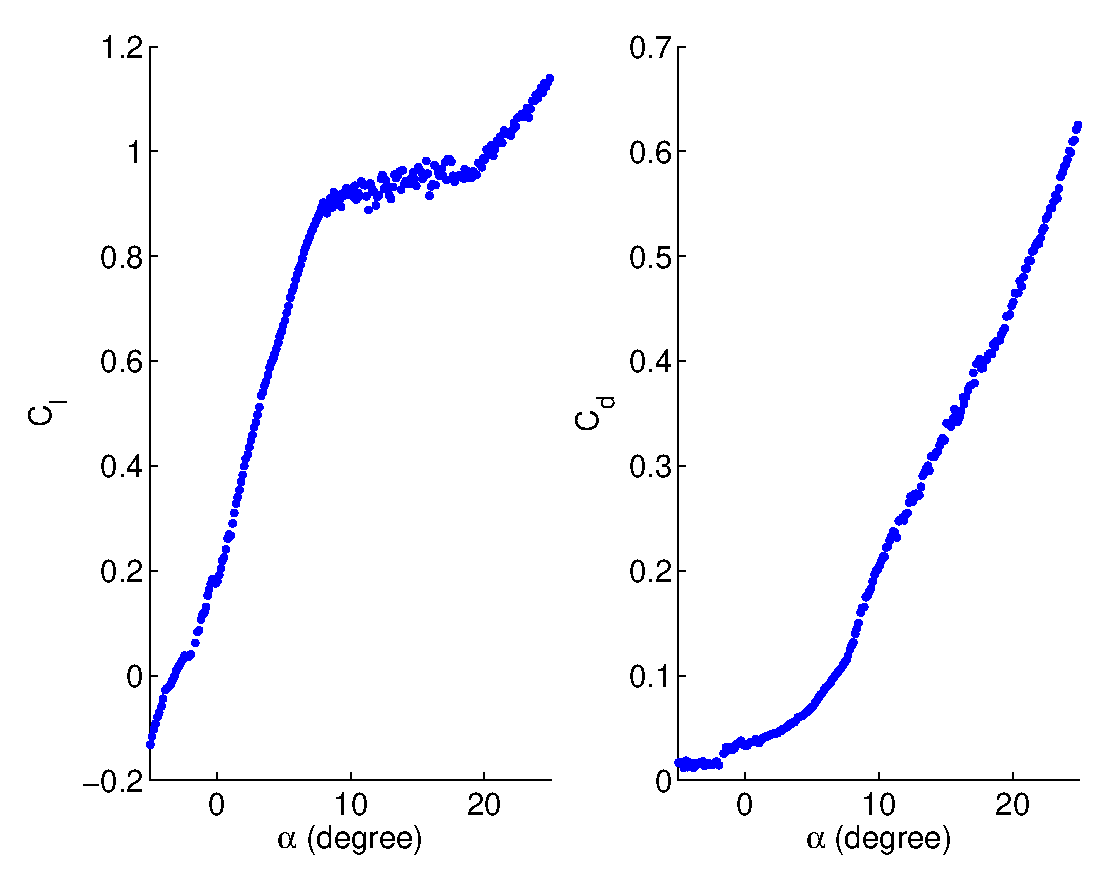
\includegraphics{./Figures/NACA0009_steady_map_Cl_Cd.eps}} 
\end{center}
\caption{Lift and drag characteristics of the NACA0009}
\end{figure}


\begin{figure}[ht]
\begin{center}
%    \scalebox{1.0}
%   {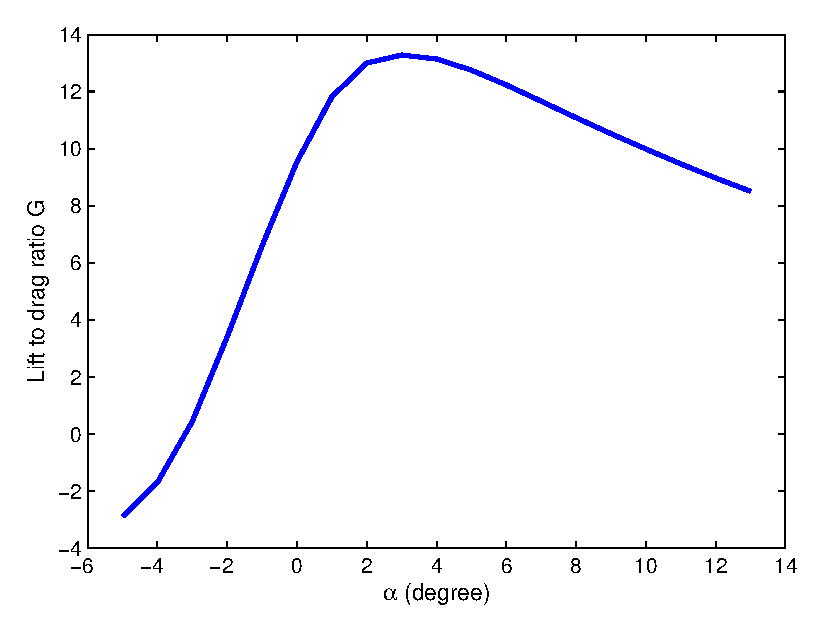
\includegraphics{./Figures/lift_to_drag_UAV.eps}}
\end{center}
\caption{Lift to drag ratio for the NACA0009}
\label{fig:G_vs_alpha_qs}
\end{figure}

\par This results, while being arguably more realistic than a simple quadratic approach, are still only considering quasi-steady change in the angle of attack.
This limitation will be discussed more in depth in the result discussion section \ref{sec:results_QS}.

\Subsection{Wind profiles}
Most of the studies done on dynamic soaring has either been done with vertical wind gusts or thermal updraft, or horizontal wind gradient foxed in time.
In this optimization procedure we chose to consider three different wind profiles made out of first order sinusoidal gusts.

\par Our first gust profile is a simple vertical gust.

\begin{equation}
\begin{array}[c]{c}
  W_g = W_a \cdot sin(2\pi T) \\
  U_g = 0 
\end{array}
\label{eqn:vertical_gust_definition}
\end{equation}

\par Similarly the horizontal gust is defined as:

\begin{equation}
\begin{array}[c]{c}
  W_g = 0 \\
  U_g = W_a \cdot cos(2 \pi T)
\end{array}
\label{eqn:horizontal_gust_definition}
\end{equation}

\par Finally a more complex combined gust is defined.
This gust profile is the sum of the two previously defined gusts.
Moreover we introduce $\phi$, a phase difference between the two component of the gust. 

\begin{equation}
\begin{array}[c]{c}
  W_g = W_a \cdot sin(2\pi T) \\
  U_g = W_a \cdot cos(2 \pi T + \phi)
\end{array}
\label{eqn:combined_gust_definition}
\end{equation}

\Section{Optimization process, cost function and constraints}

\Subsection{General consideration on optimization}
% Get some stuff from the MM544 class
The general principle for the optimization routines resides in defining a so called ``cost function'' that will represent a quantity we want to minimize.
While the algorithm tries to minimize this scalar, a set of constraints have to be respected. 
These constraints can represent physical limitations or specific requirements related to the system at hand.
The cost and constraints are expressed as functions of a set of system state variables.
The state variables can represent temporal or spatial values.
The optimization is performed in a sequential fashion where different algorithm are used to step from one set of values for the state variables to another. 

\par Optimization routines are divided into two families. 

\par The first method is called the gradient method, it requires a good knowledge of the physics behind the problem.
The cost function as well as the constraints have to be explicitly defined.
In this method the gradient of the cost function and the constraints is used to determine the direction of the next step in the optimization.
Different algorithm are used to chose the step size, and sometime the direction of the previous step can influence the current step.
The gradients for either the cost function or the constraints do not have to be explicitly defined as modern optimization routines, such as the one included in Matlab, can perform numerical gradient estimation.
However inputting an user defined gradient into the routine will significantly speed up the overall process.

\par The second method is using the so called ``evolutionary algorithms''. 
This method relies a lot less on knowing the underlying physical phenomenon.
Its basic principle is a ``try and see'' process.
Random changes are performed on the state variables and their effects on the cost function are assessed.
The best steps are selected as a starting point for the next generation.
While with this method each step is a less computation intensive than with the previous method, the number of steps is a lot higher.

\par The first method has been used in this optimization as it provides more insight on the physics behind the problem.
However it should be noted that the resulting ``optimal'' point is usually only assured to be \emph{a local} minimum of the cost function.
Several different starting states should be tested to ensure that the optimization converges toward a reasonable minimum.



\Subsection{Cost function}
Our problem here consists in optimizing the trajectory in a gusting environment to minimize energy lose.
The most obvious cost function would be something like

\begin{equation}
  - \frac{1}{2}m{V(T_f)}^2 - gX(T_f)
  \label{eqn:eni_cost_fun}
\end{equation}

Which would be equivalent to maximizing the total energy at the end of the gust.
However after testing this has shown to leave to much freedom to the algorithm. 
As a result the local minimum found are the result of trajectories such as very steep dives, clearly far from the optimum.

\par Once again we refer to the Lissaman paper \cite{Lissaman2007neutral} and chose, instead of minimizing energy loss for a given gust condition, to find the minimum gust amplitude to satisfy an energy neutral trajectory over the gust period.
This means that the cost function is the wind gust amplitude, which will have to be added to the state vector in order to be explicit, and that the neutral energy trajectory will have to be added to the constraints

\Subsection{State vector and constraints formulation}
In our case a gust cycle of duration $T_f$ is divided into $N$ discrete instants $T_i$ (usually between 31 and 101).
At each of these points we need to know the state of the vehicle.
Since we are considering a two degree of freedom model the two positions $X$, $Z$ and speed $U$, $W$ variables are the most simple choices.
However this is not enough to describe the system completely, we also need to know what our input is going to be, in this case the lift available and where on the lift vs drag curve we are.
Theres is two possible choices for this.
If you consider only the quasi steady part, the angle of attack $\alpha$ seems obvious.
However since the drag is a function of the lift (the inverse is not true), it is possible to use only the $L$ to define our point on the lift to drag curve.
This allows us to use one less variable.

\par With this five variables defined at each considered time points the state and input vector look like:

\begin{equation}
  x= 
  \begin{bmatrix}
    \cdots \\
    X_i \\
    Z_i \\
    U_i \\
    W_i \\
    L_i \\
    \cdots \\
    W_a
  \end{bmatrix}
  \quad i \in [1,N]
  \label{eqn:big_vector}
\end{equation}

\par All this variables have to be constrained to achieve a realistic trajectory.
The first and most obvious constrain is done with the equation of motion \ref{eqn:non_dim_eqm}.
This equation has to be changed from a continuous differential equation to a discrete equation.
This is done by using the Simpson's 1/3rd rule as derived by Zhao \cite{zhao2004optimal}.

In order to satisfy the equations of motion we need to define the state variable at the time $T_i$:

\begin{equation}
  y_i= \begin{bmatrix}
    X_i \\
    Z_i \\
    U_i \\
    W_i 
  \end{bmatrix}
  \label{eqn:state_i}
\end{equation}

Then with $\dot{y_i}$ the derivative of the state variables, given by the equation of motion \ref{eqn:non_dim_eqm} and:

\begin{equation}
  \begin{array}[c]{c}
    y_m= \frac{1}{2}(y_k + Y_{k+1}) - \frac{1}{8}(\dot{y_{k+1}} - \dot{y_k})\delta t \\
    L_m=\frac{1}{2}(L_i + L_{i+1})
  \end{array}
  \label{eqn:simpson_middle}
\end{equation}

The condition to satisfy the equation of motion becomes

\begin{equation}
  0=y_{k+1} - y_k - \frac{1}{6}( \dot{y_k} + 4 \dot{y_m} + \dot{y_{k+1}})\delta t \quad \forall i \in [1,N-1]
  \label{eqn:simpson}
\end{equation}

\par Another constraint is on the neutral energy loop condition.
To account for that the initial and final $Z$ values are fixed at zero and the initial and final vertical and horizontal speeds are set to be equal.

\par Since we are looking at only one cycle, in order for it to be repeatable, we need to have a smooth transition from one to another.
This  means setting the derivative of the speed to be equal at the start and at the end of the cycle.

\begin{equation}
  \begin{array}[c]{c}
    W_2 - W_1 = W_N - W_{N-1} \\
    U_2 - U_1 = U_N - U_{N-1} 
  \end{array}
  \label{eqn:derivative_constraint}
\end{equation}

\par Finally the last set of constraint is on the physical limits of the aircraft.
Typically an aircraft flight envelope is limited by its maximum speed (depends on the dynamic pressure), its maximum load and its maximum lift (which determines the stalling speed).
Since our aircraft is will be flying around its optimal glide speed, over speeding isn't going to be an issue.
Moreover the drag increasing proportionally to the square of speed, high speeds will be avoided as much as possible by the optimization routine.
The limit on the load can conveniently be expressed as:

\begin{equation}
  L_i Q_i \leq g_max \quad \forall i \in [1,N]
  \label{eqn:load_constraint}
\end{equation}

With $g_max$ the maximum load in Gs.

% did I actually used that in my code? I think it wasn't necessary.

\par Finally the maximum lift condition can be expressed

\begin{equation}
  L_i \le \frac{C_l^{max}}{C_l^*} \quad \forall i \in [1,N]
  \label{eqn:lift_constraint}
\end{equation}

As it will be seen in section \ref{sec:results_QS} the value of $C_l^{max}$ has a profound impact on the performances of the UAV.

\par It is also sometime advisable to limit $\gamma$ in the $\pm 90^{\circ}$ range to prevent loops and backtracking.


\Subsection{Matlab optimization function}
Matlab offers several ways of doing optimization.
Since this scripting language allows for easy parallelization, it is relatively painless to implement your own optimization code.
However in most cases, ``classical'' optimization problems, such as weight reduction, topology optimization or mechanism design are reducible to a set of linear  equations and constraints.
In our case the equations of motions as well as the lift and drag properties are not linear at all, and trying to linearize this problem would make any solution meaningless.
For this reason a already existing optimization function has been chosen.

\par Since non linear optimizations like that are a computation intensive process dedicated tools have been developed to tackle the problem.
SNOP is one of these software and seems to be widely used.
Another tool appearing in the literature is a Fortran library called NPSOL.
Since our laboratory's language of predilection is Matlab, the optimization toolbox from MathWorks was used.

\par The optimization toolbox provides with a helpful function for non-linear optimization called \emph{fmincon()}.
This function needs an initial guest for the $x$ vector.
When using this function the initial guest has quite a big influence on the converging speed and on the local optimal solution found.
To account for that several educated guesses were made and tested for the different types of the wind profiles and gusts duration.
These guesses are refined as new results are obtained.


\Section{Results for quasi-steady aerodynamics} \label{sec:results_QS}

\Subsection{Implementation validation}
The first step is to validate the code implemented here against previous results. 
Even if the lift and drag profiles are different from Lissaman's assumptions a similar case is optimized.
The gust duration is set to be $T_g=4 T$, for a purely vertical gust.
Since it is only a validation test the same lift and drag characteristics are used. Equation \ref{eqn:Lissaman_G} plugged into the equation of motion part of the code. An optimal lift to drag ratio of $G_{max}=20$ is chosen, as seen in the original Lissaman paper \cite{Lissaman2007neutral}.

\begin{figure}[ht]
  \begin{center}	
    \scalebox{1.0}
    {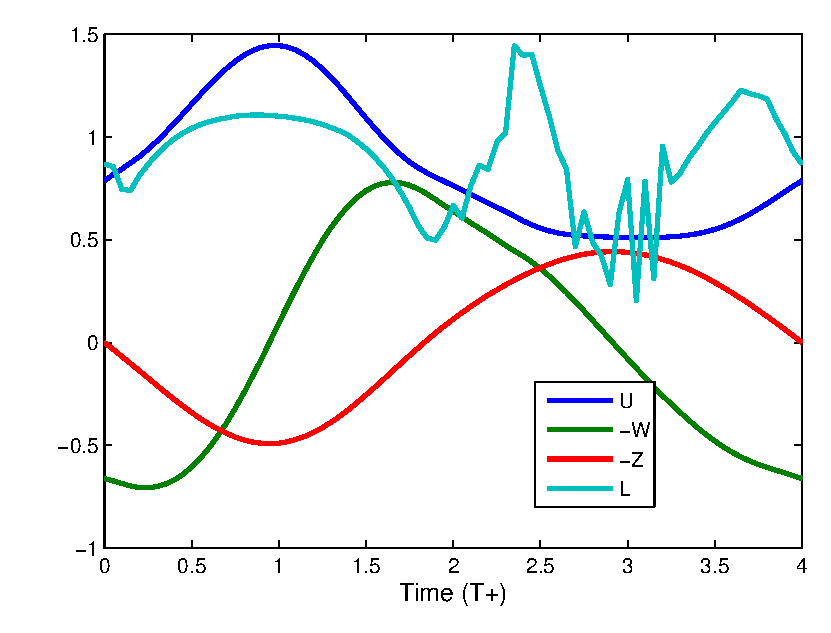
\includegraphics{./Figures/Windtype=1_Tg=4_Wg=0p129_quad_G=20.eps}}
  \end{center}
  \caption{Optimization results for a $4T$ long vertical gust}
  \label{fig:Validation_optimization}
\end{figure}

\FloatBarrier

Lissaman, with is optimal lift to drag ratio of 20 found a wind gust amplitude of $0.129$. 
Here the minimum required for neutral energy loop is $0.128$ (see figure \ref{fig:Validation_optimization}).
The shape of the state and control parameters curves are also consistent with the Lissaman results.

\par Similarly an optimization is performed for a purely horizontal wind gust.

\begin{figure}[h]
  \begin{center}
    \scalebox{1.0}
    {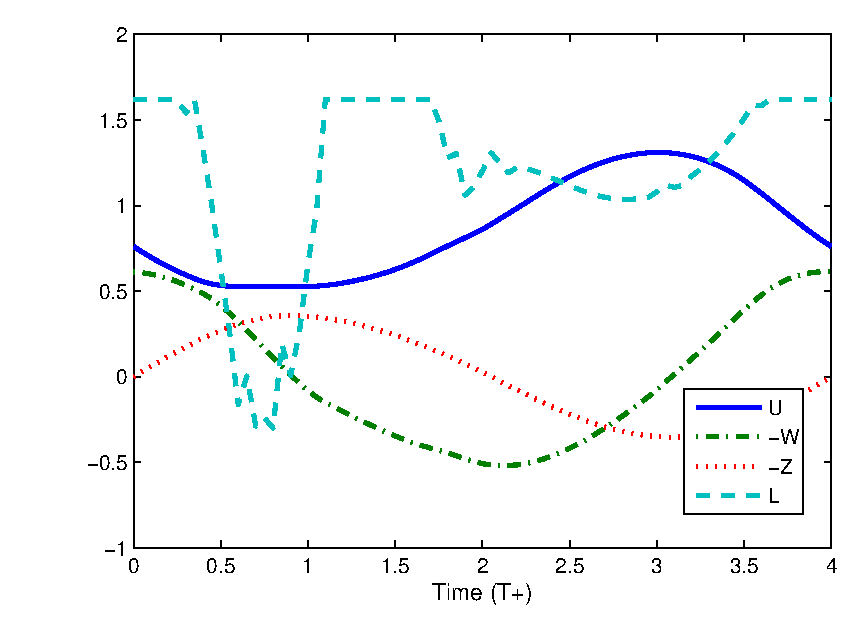
\includegraphics{./Figures/Windtype=2_Tg=4_Wg=0p246_quad_G=20.eps}}
  \end{center}
  \caption{$4T$ long horizontal gust for $G=20$, $W_a=0.246$}
  \label{fig:Horizontal_optimization}
\end{figure}

The resulting minimum wind amplitude is higher than for the vertical gust. 
However this shows that it is possible to take advantage of horizontal wind gusts to save energy if the performances are high enough.

\par Finally a combined horizontal and vertical gust is simulated.

\begin{figure}[h]
  \begin{center}
    \scalebox{1.0}
    {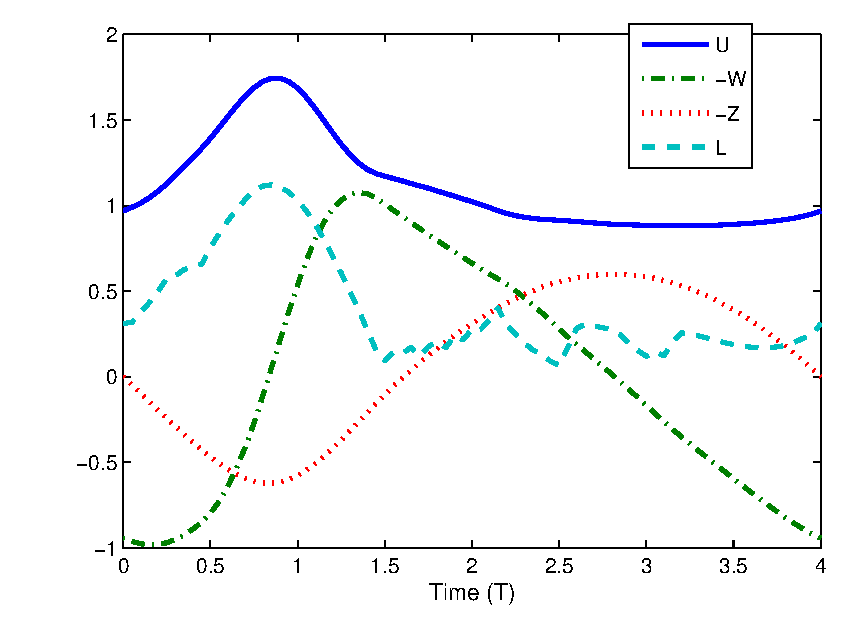
\includegraphics{./Figures/Windtype=3_Tg=4_Wg=0p232_quad_G=20.eps}}
  \end{center}
  \caption{$4T$ long combined gust for $G=20$, $W_a=0.232$}
  \label{fig:combined_optimization}
\end{figure}

Unsurprisingly the neutral energy loop trajectory exists also for this case.

\FloatBarrier

\Subsection{Typical results for the NACA0009 wing}

\par A similar batch of optimizations is done with the more realistic lift and drag profiles.

\begin{figure}
  \begin{center}
   \scalebox{1.0}
   {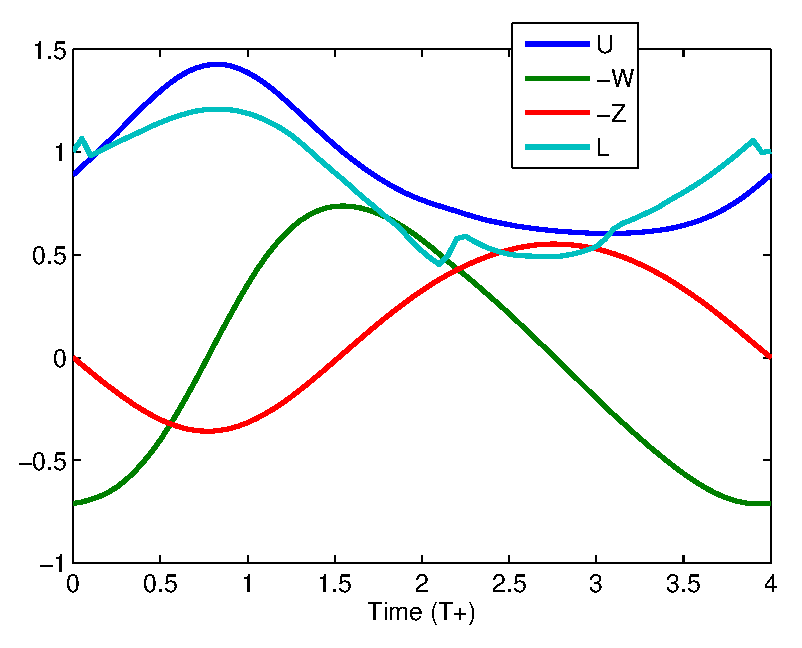
\includegraphics{./Figures/Windtype=1_Tg=4_Wg=0p205_UAV_alphamax=12.eps}}
  \end{center}
  \caption{$4T$ long vertical gust for UAV, $W_a=0.205$}
  \label{fig:vertical_optimization_UAV}
\end{figure}


\begin{figure}[h]
  \begin{center}
    \scalebox{1.0}
    {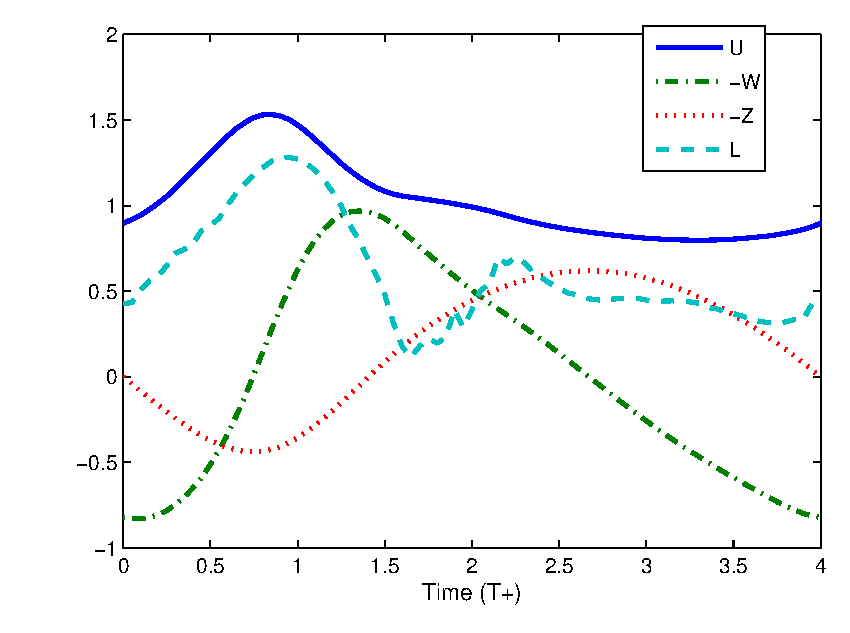
\includegraphics{./Figures/Windtype=3_Tg=4_Wg=0p387_UAV_alphamax=12.eps}}
  \end{center}
  \caption{$4T$ long combined gust for UAV, $W_a=0.387$}
  \label{fig:combined_optimization_UAV}
\end{figure}
\FloatBarrier

As it can be seen on the figures \ref{fig:vertical_optimization_UAV} and \ref{fig:combined_optimization_UAV} the trajectories are similar in shape. However the gust amplitude needed to achieve neutral energy flight are a lot higher.
Such differences can be explained by looking at the maximum lift to drag ratio for both conceptual aircraft.
The quadratic drag profile used by Lissaman has a $G_{max}$ of 20.

\FloatBarrier

\par With this kind of performances, a purely horizontal gust can't sustain a neutral energy loop.

\FloatBarrier

%\par Now that we have shown that for each type of trajectories the general behavior is the same, independently of the lift to drag ratio, it is interesting to compare at what time the energy was gained and at what rate it was changing.
%
%\par In the following figure the potential energy and kinetic energy are dissociated to highlight the actual effects of the altitude and speed gain.

% Do I want to make a trajectory/vector graph ??


\Subsection{Influence of the gust duration}
From our literature review it seems like most of the studies done on gusting winds has been conducted on gusts duration greater than $2T$.
Considering shorter gusts seemed unreasonable since only quasi steady aerodynamic models were used. 
However since the purpose this research is to extend the energy extraction envelope, such cases should be considered.

\begin{figure}[h!]
  \begin{center}
    \scalebox{1.0}
    {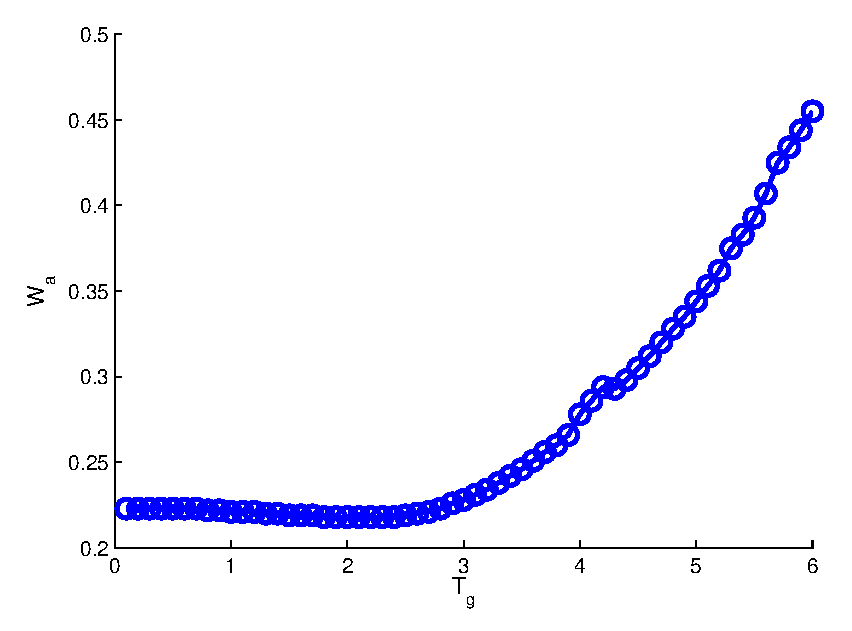
\includegraphics{./Figures/Wg_vs_TG_windtype=1_alhpamax=12_nodalphalimit.eps}}
  \end{center}
  \caption{Influence of gust duration on the minimum gust amplitude for vertical gusts}
  \label{fig:vertical_amplitude_duration}
\end{figure}

\begin{figure}[h!]
  \begin{center}
    \scalebox{1.0}
    {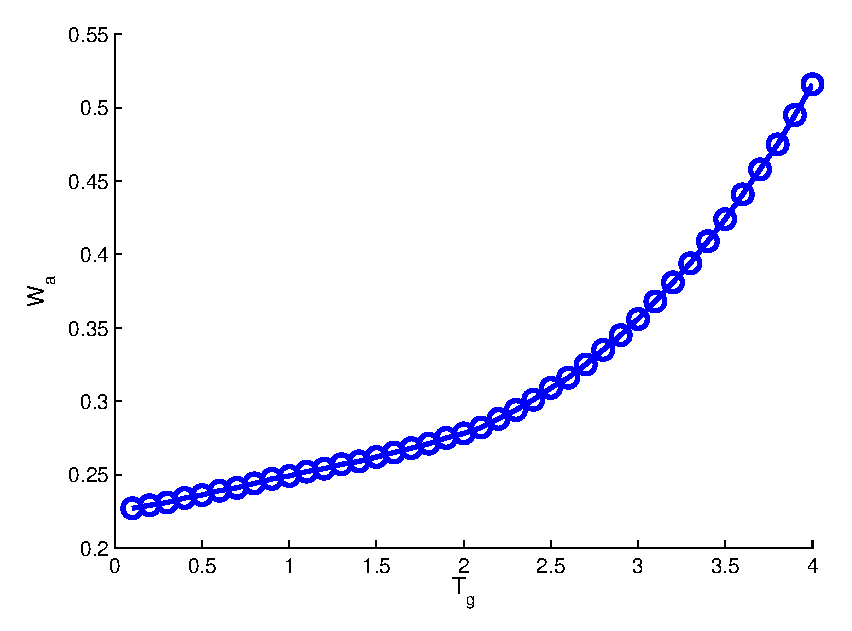
\includegraphics{./Figures/Wg_vs_TG_windtype=3_alhpamax=12_nodalphalimit.eps}}
  \end{center}
  \caption{Influence of gust duration on the minimum gust amplitude for combined gusts}
  \label{fig:combined_amplitude_duration}
\end{figure}

\par Interestingly shorter gusts require less wind amplitude than the long ones.
This seems to indicate that most of the lost energy is due to the non-conservative drag force and not due to the downwind effects.
However the actual minimum gust amplitude required for neutral energy flight has a minimum for $2.5T$ long vertical gusts.

\par In figure \ref{fig:combined_amplitude_duration} This time no minimum is found.
This seems to reinforce the idea that the losses are mainly due to the energy dissipated by the drag since in this case the drag influence is mitigated by the horizontal component of the combined gust.

%\par The diminishing gust amplitude required is an interesting phenomenon but can be fairly easily explained.
%For a glider the only energy dissipation comes from the drag, in the cases we are considering the energy loss can be seen as a superposition of the losses due to simple cruse flight and the ones due to the maneuvering.
%Since the total flight time during short gusts is shorter while the relative wind velocity remains more or less constant, the energy loss due purely to flying this long should be proportional to the flight time.
%The energy input for this system is the wind gust itself is proportional to the force on the fluid times its velocity and the gust duration.
%Since the force required to move the fluid is itself proportional to the derivative of the gust velocity the energy of the gust over a whole gust is in fact only proportional to the square of the gust amplitude.
%
%\par This means that if the energy extraction efficiency was constant the value of $\frac{T_g0}{{W_g0}^2}$ should be constant for all the cases.
%
%
%\begin{figure}[h!]
%  \centering
%  %\includegraphics{<+file+>}
%  \caption{Energy extraction effectiveness}
%  %\label{fig:<+label+>}
%\end{figure}
%


\FloatBarrier

\par To understand the difference between the short gusts ($T_g \leq 3$) and the long gusts ($T_g \geq 3$) a closer look at the profile of the angle of attack over time is needed.


\begin{figure}[h]
  \centering
  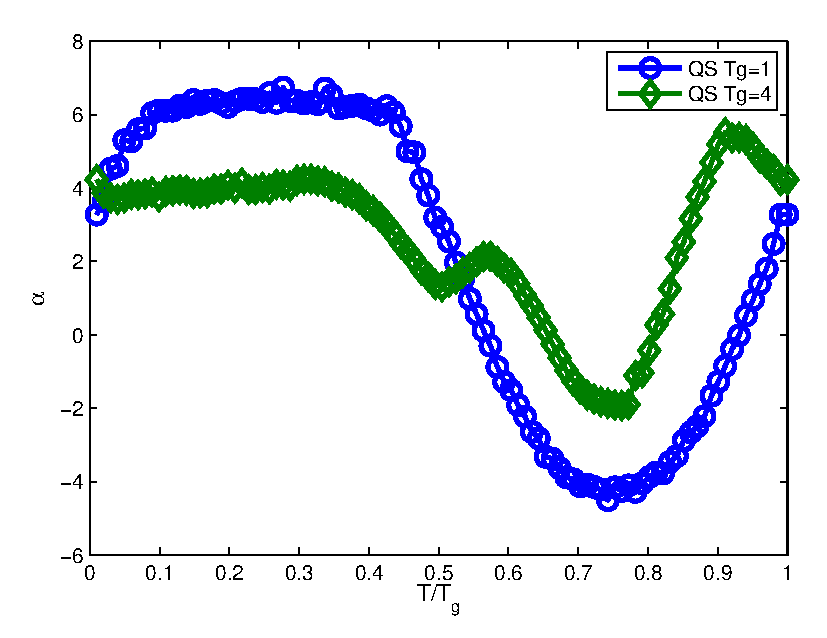
\includegraphics{./Figures/alpha_vs_Tg_QS_short_vs_long_wt1.eps}
  \caption{Difference between short and long gust angle of attack profile for vertical gusts}
  \label{fig:short_vs_long_qs_wt=1}
\end{figure}

\begin{figure}[h]
  \centering
  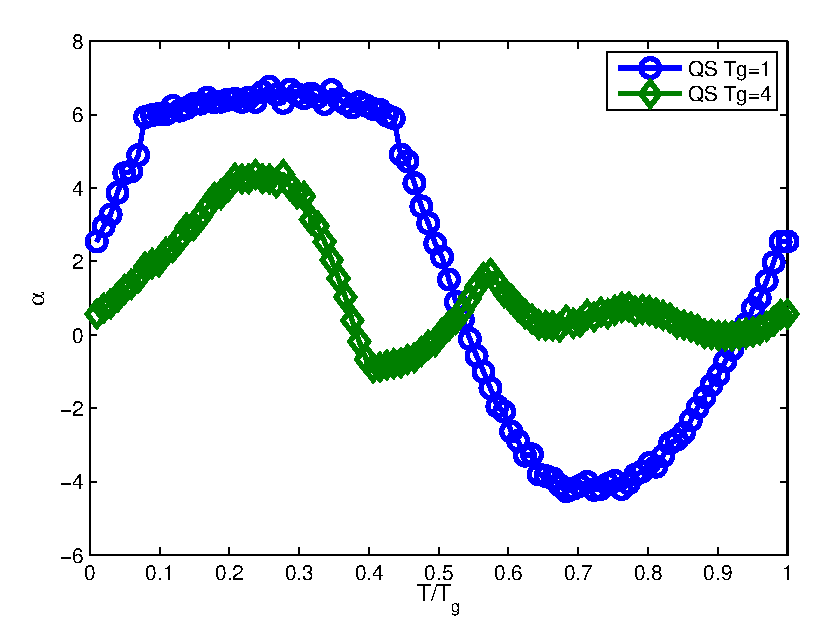
\includegraphics{./Figures/alpha_vs_Tg_QS_short_vs_long_wt3.eps}
  \caption{Difference between short and long gust angle of attack profile for combined gusts}
  \label{fig:short_vs_long_qs_wt=3}
\end{figure}

\par Figures \ref{fig:short_vs_long_qs_wt=1} and \ref{fig:short_vs_long_qs_wt=3} shows the clear distinction between short and long gusts results.
These profiles are representative of what happens left and right of the $T_g=3$ value.

\par For longer duration gust the amplitude needed from the lift appears to be reduced, the algorithm seems to minimize the drag losses by flying close to either the maximum lift to drag ratio ($\alpha = 3.5 ^{\circ}$) or the minimum drag point at the zero angle of attack point.
Only a short period of negative lift is needed.

\par Shorter gusts need more amplitude to achieve the energy neutral loop.
The angle of attack saturates at around $6^{\circ}$ and its minimum also decreases.
The value of 6 degrees correspond to were the lift to drag ratio starts to really dip (see figure \ref{fig:G_vs_alpha_qs} so it is probable that the optimization routine voluntarily avoids these high drag regions. 


% get some commentary there
\FloatBarrier
\Subsection{Influence of phase variation in the combined gust case}
\emph{IS KEEPING THIS PART INTERESTING???}
For combined vertical and horizontal gusts another parameter can be changed.
So far the phase between the two components of the gust has been constant.

\par For this we define the phase $\phi$ as:

\begin{equation}
  \begin{array}[c]{c}
    W_g=W_a cos(2\pi T) \\
    U_g=W_a sin(2\pi T + \phi)
  \end{array}
  \label{eqn:combined_gust_phase}
\end{equation}

After Simulations are performed by 10 degrees steps with the following results.

\begin{figure}[ht]
  \begin{center}
    \scalebox{1.0}
    {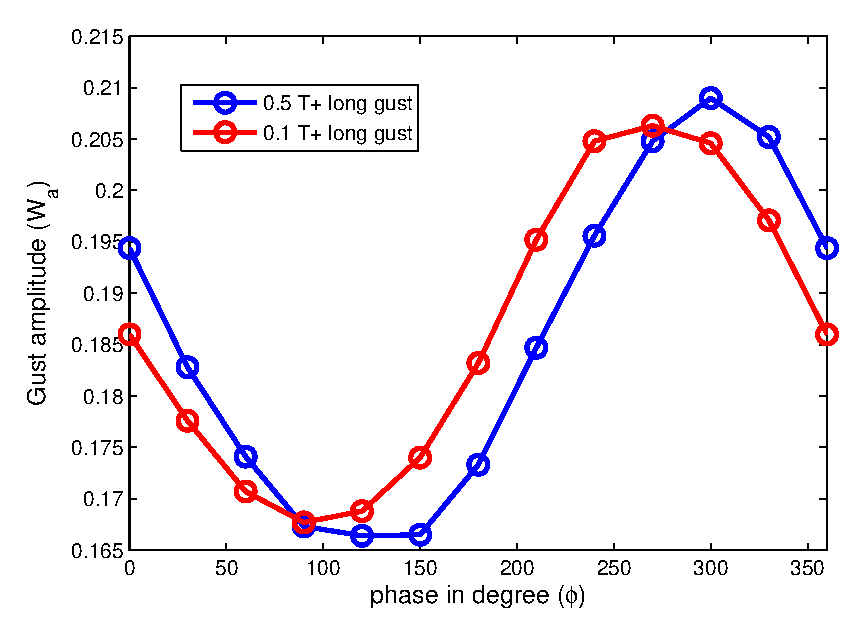
\includegraphics{./Figures/combined_gust_amplitude_vs_phase.eps}}
  \end{center}
  \caption{Influence of the phase between the component of the combined gust}
  \label{fig:combined_amplitude_phase}
\end{figure}

\par This clearly shows that our minimum gust amplitude for a 0 phase was actually close to the worst case possible.
The best case scenario is when the phase is around 90 to 120 degrees and the worst is around 270 to 300.

\FloatBarrier

\par We can see that the results are different for different gust durations.
One possible explanation for this is that at some point the inertia is too great and start to act as a low pass filter, introducing some phase shift in the trajectory. 

\Subsection{Effects of the maximum angle of attack allowed}
The previous results show that for shorter gusts higher values of the angle of attack much be reached.
The issue is that higher angle of attacks can get dangerously close to region where the flow is separated.
To make sure no separation happens a new linear constraint is put on the angle of attack.
The angle is limited to a range of $\pm 5 ^{\circ}$, the linear part of the lift curve.


\begin{figure}[h]
  \centering
 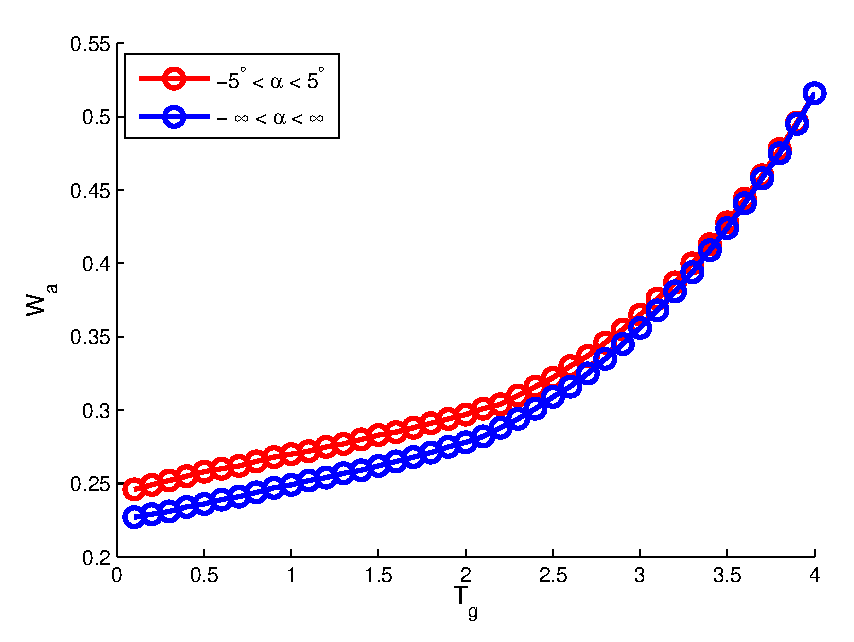
\includegraphics{./Figures/allowed_alpha_wg_tg_wt=3.eps}
  \caption{Difference in performance for combined wind gusts if no high angle of attack are allowed}
  \label{fig:allowed_alpha_Wt_vs_tg_wt=3}
\end{figure}

\begin{figure}[h]
  \centering
 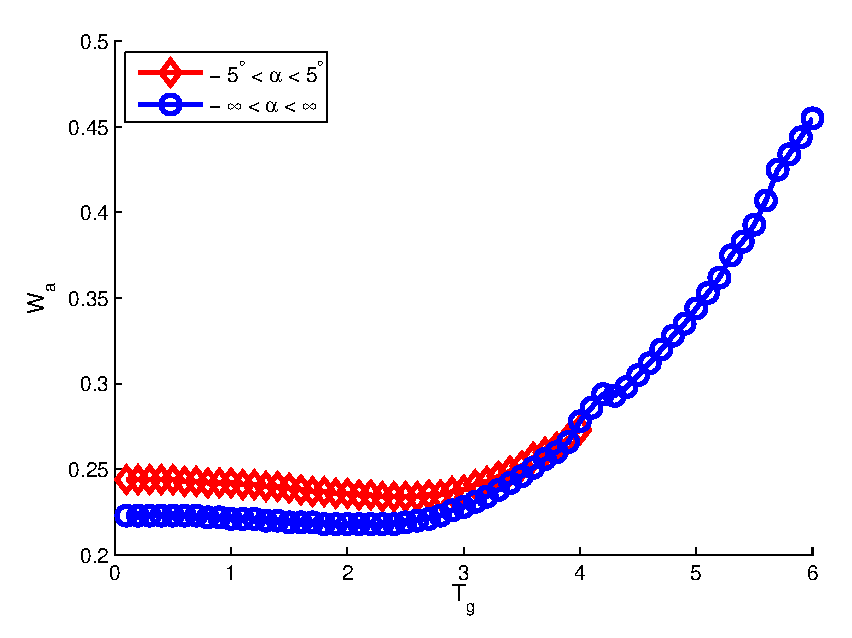
\includegraphics{./Figures/allowed_alpha_wg_tg_wt=1.eps}
  \caption{Difference in performance for vertical wind gusts if no high angle of attack are allowed}
  \label{fig:allowed_alpha_Wt_vs_tg_wt=1}
\end{figure}

\FloatBarrier

As seen here the results are confirming the previous analysis of the difference between short and long gusts.
There is no difference in the longer gusts region because, as seen before the optimization results in no angle of attack bigger than $4^{\circ}$.
The difference is that for shorter gusts duration the more violent maneuvers are not available anymore.
It can be seen on figure \ref{fig:alpha_vs_tg_maxalpha=5} that the angle of attack comes right against the limit of 5 degrees.

\begin{figure}[h]
  \centering
  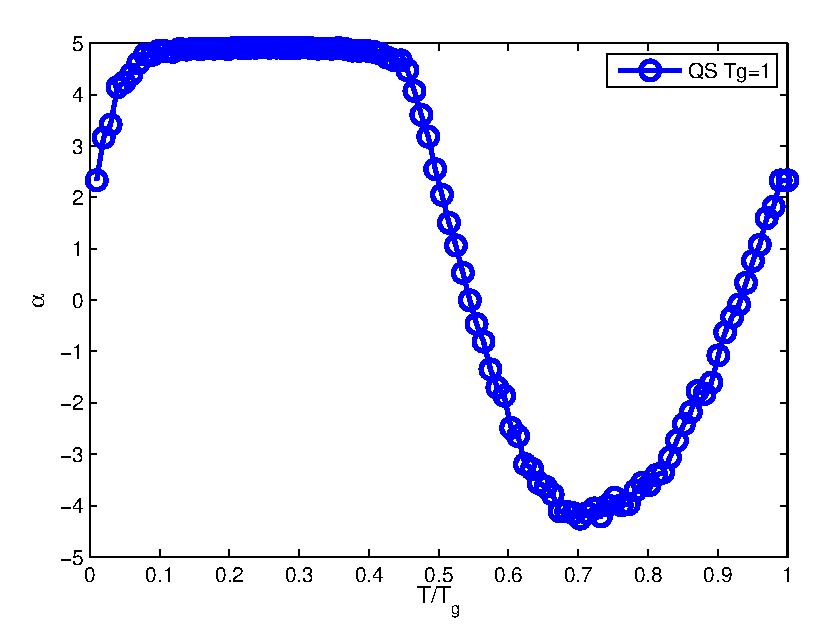
\includegraphics{./Figures/alpha_vs_tg_Tg=1_wt3_maxalpha=5.eps}
  \caption{Result of limiting the angle of attack to $5^{\circ}$ for $T_g=1$ in a combined gust}
  \label{fig:alpha_vs_tg_maxalpha=5}
\end{figure}

\FloatBarrier
\Subsection{Additional remarks}
Analyzing each of the solutions found, and notably the non optimal ones it can be see, as noticed by Lissaman, that the exact shape of the lift input isn't really important.
In his paper he approximated the input with a simple sinusoidal curve with amplitude and phase control, similar inputs in this simulation have produced minimum gust amplitude similar to the previous results.
This raises the hope that even very basic controllers should be able to improve UAV endurance as a very precise control of the lift and drag are not required to get improvement oer a non-controlled case.

% [DO I WANT TO  CHANGE THE PHASE TO ACTUALLY TEST IT !!!!]
\par While these results are supposed to be the optimal solution, it does not mean a controller can achieve such performances.
Even if the trajectory and lift curves are physically possible, the optimization algorithm assume a known gust shape and optimize all of the time points at once.
This means that contrary to a real controller the optimized trajectory can anticipate the wind change and preemptively react.
Even if the wind gusts were perfectly sinusoidal, it would not be able to anticipate since a controller is casual.
Finally in a real life scenario the wind would of course not be a simple clean sinusoidal gust.

\par The simulation is also limited by its inability to account for the moment of inertia along the pitch axis.
Fast pitching as seen for shorter gusts would require a huge amount of pitch authority.

\par Even with all this limitations these results provide good insight into what would be needed implement energy extraction trajectories in UAVs.


